% ==========================================================================
% INFO 4617 Web Data Science -- Week 9: Extracting Data from PDFs (Chapter 9)
% Build:  latexmk -pdf week-09.tex   (from this folder; no env vars needed)
% (or run `make` from the slides/ directory to build every deck)
% ==========================================================================
\documentclass[9pt,aspectratio=169]{beamer}
% Resolve the shared theme/preamble in ../common/ when compiling this
% file directly from its own folder (no TEXINPUTS needed).
\makeatletter\def\input@path{{../common/}}\makeatother
\input{preamble}

\title[Week 9 · PDFs]{{\Huge Extracting Data from PDFs}}
\subtitle{Week 9 · Documents module · Textbook Chapter 9}
\author[Keegan]{\textbf{Brian C. Keegan, Ph.D.} \\ Associate Professor, Department of Information Science \\ University of Colorado Boulder}
\date{October 12, 14 \& 16, 2026}

\begin{document}

\maketitle

% -------------------------------------------------------------------------
\begin{frame}{This week at a glance}
    PDFs are the web's filing cabinets. This week we pry official records out of them and turn locked documents into data.

    \bigskip

    \dayband{Monday}{Concepts \& notebook intro}
    \begin{itemize}\small
        \item Why PDFs resist extraction; reconstruction vs.\ reading
        \item Text layers and OCR; getting text out by hand, from readers, office tools, and the command line
        \item In class: the city's revenue report, by hand (20 minutes)
    \end{itemize}

    \medskip

    \dayband{Wednesday}{Notebook lab}
    \begin{itemize}\small
        \item Work the Chapter 9 notebook: pypdf on the council minutes, pdfplumber on the revenue reports
    \end{itemize}

    \medskip

    \dayband{Friday}{Textbook revisions}
    \begin{itemize}\small
        \item Propose \& peer-review pull requests improving Chapter 9
    \end{itemize}
\end{frame}

\begin{frame}{Course overview}\centering
    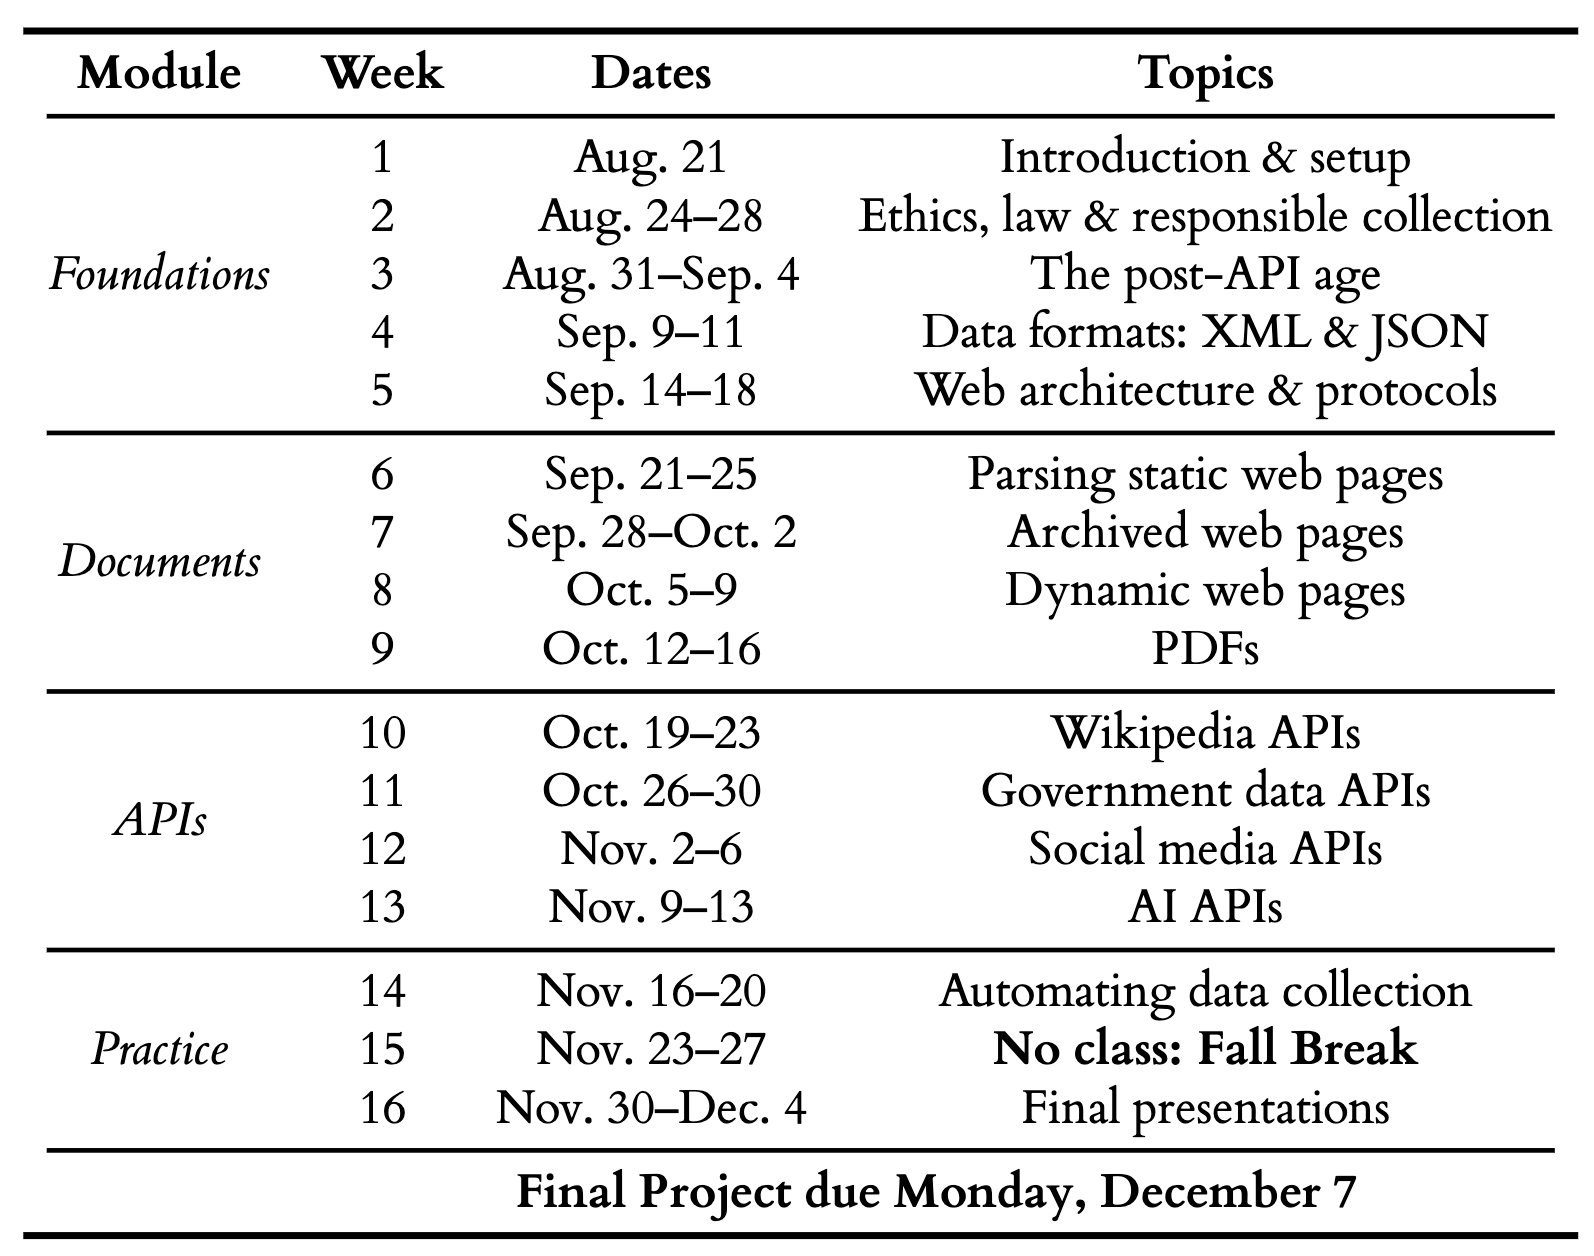
\includegraphics[width=.67\textwidth]{slides/common/course-overview.png}
\end{frame}

% =========================================================================
\section{Monday · Concepts}
% =========================================================================

\begin{frame}{The web's filing cabinets}
    \begin{columns}[T]
        \begin{column}{0.55\textwidth}
            PDFs are everywhere in institutional record-keeping: council minutes, bill texts, financial reports, court filings, academic papers, environmental impact assessments.

            \bigskip

            They are the format of choice for ``official'' documents because they \textbf{preserve visual layout} across any device or printer. But that priority --- visual fidelity over semantic structure --- makes them \textbf{hostile to programmatic extraction}.

            \bigskip

            The records inside are \textit{readymade} data (\textcite{salganik2018bit}). Somebody made them for administration, not for research. With effort you can still use them to answer questions that their authors never expected.
        \end{column}
        \begin{column}{0.4\textwidth}
            \centering
            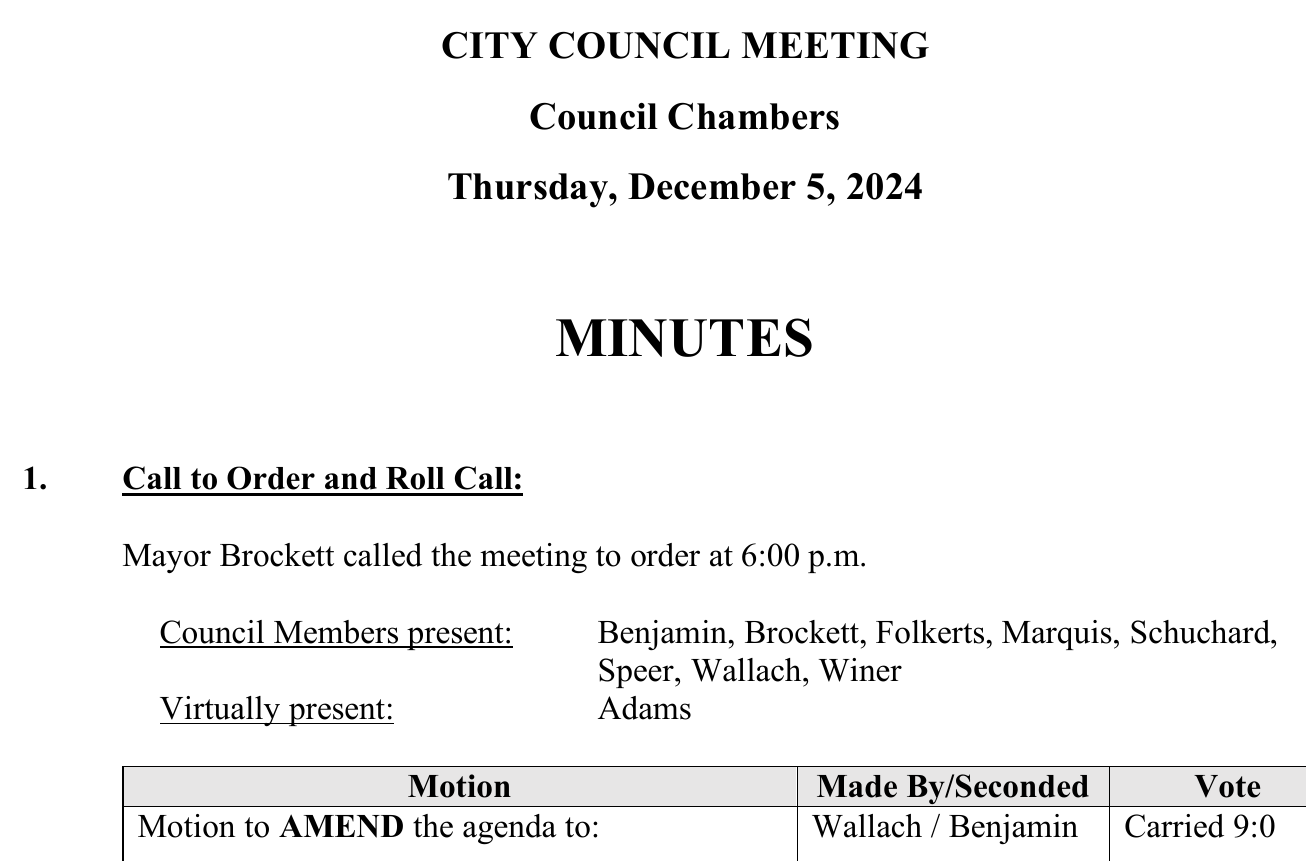
\includegraphics[width=\textwidth]{img/council_minutes_pdf.png}\\
            {\scriptsize Boulder City Council minutes, December 5, 2024: the roll call on page 1.}
        \end{column}
    \end{columns}
\end{frame}

\begin{frame}{A computer never reads a PDF}
    \begin{columns}[T]
        \begin{column}{0.46\textwidth}
            When \textbf{you} read a PDF you see paragraphs, tables, headers, and page numbers.

            \bigskip

            A \textbf{computer} reads a different thing. It sees a sequence of drawing instructions: \textit{put this character at $(x, y)$. Draw a line from here to there. Add this image}.

            \bigskip

            So text extraction is \textbf{reconstruction, not reading} --- the computer must infer logical structure from spatial layout. The results will not be perfect, but they can be good enough to turn inaccessible records into analyzable datasets.
        \end{column}
        \begin{column}{0.5\textwidth}
            \centering
            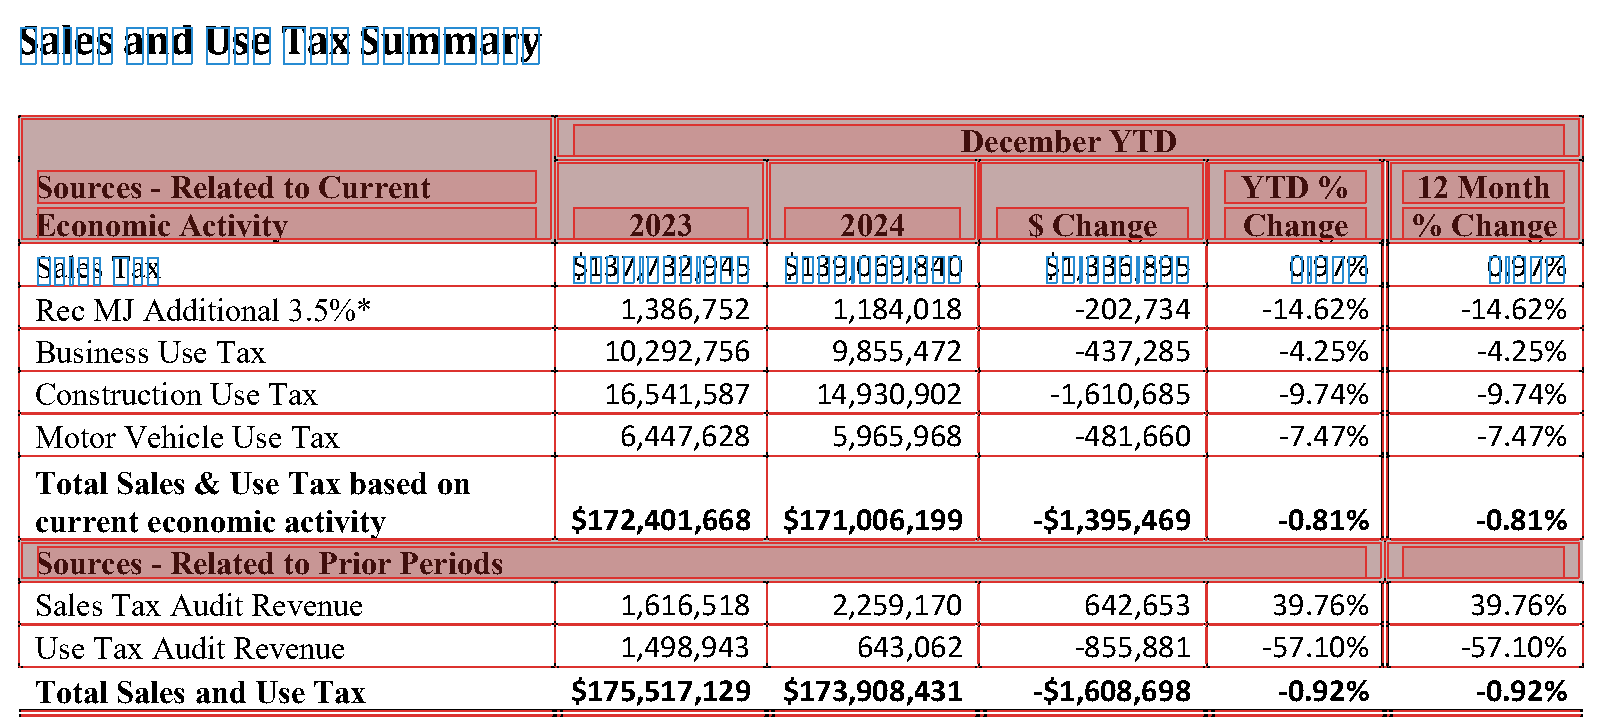
\includegraphics[width=\textwidth]{img/pdf_drawing_instructions.png}\\
            {\scriptsize Boulder's December 2024 revenue report, as pdfplumber sees it: each character placed on its own (blue boxes, two rows shown), and the table's lines are 290 thin rectangles (red).}
        \end{column}
    \end{columns}
\end{frame}

\begin{frame}{Getting text and data out of a PDF}
    \begin{columns}[T]
        \begin{column}{0.48\textwidth}
            \begin{itemize}\small
                \item \textbf{Text layer} --- the characters a PDF stores, each with a font and a position. Select it, search it, copy it.
                \item \textbf{Born-digital PDF} --- saved from Word, Excel, or a web page. It has a text layer.
                \item \textbf{Scanned (image-only) PDF} --- photographs of paper pages. No text layer: nothing to select.
                \item \textbf{OCR}, optical character recognition --- software that recognizes letters in an image and writes them out as text. \textbf{Tesseract} is the free, open-source engine most tools use.
            \end{itemize}
        \end{column}
        \begin{column}{0.48\textwidth}
            \begin{itemize}\small
                \item \textbf{Searchable PDF} --- the page image with an invisible OCR text layer on top. \texttt{tesseract} makes one from a page image.
                \item \textbf{Layout analysis} --- working out columns, reading order, headers, and footers from where text sits.
                \item \textbf{Table extraction} --- rebuilding rows and columns from lines and positions. Tabula, \texttt{pdfplumber}, \texttt{camelot}.
                \item \textbf{Handwriting recognition} (HTR) --- OCR for handwriting. Much less accurate than print.
                \item \textbf{Document AI} --- a vision-language model reads the page image and writes text or a table. Fast and fluent, and it can invent what it can't read: check it against the page.
            \end{itemize}
        \end{column}
    \end{columns}
\end{frame}

\begin{frame}{First, by hand: readers and office tools}
    Try this before you write code. One table, once, rarely needs Python.

    \medskip

    \begin{itemize}\small
        \item \textbf{Is there text?} Drag across a line, or search with Ctrl+F (Cmd+F). If nothing highlights, it's a scan: go to OCR.
        \item \textbf{Copy and paste} from any reader. Paragraphs come through. A table arrives as runs of text that you split into columns yourself.
        \item \textbf{Adobe Acrobat Reader} (free): \textit{File $\to$ Save As Other $\to$ Text}. Export to Word or Excel needs a paid Acrobat subscription.
        \item \textbf{Microsoft Word}: \textit{File $\to$ Open} a PDF, and Word converts it to an editable document. Best on PDFs that are mostly text.
        \item \textbf{Microsoft Excel} (Microsoft 365, Windows): \textit{Data $\to$ Get Data $\to$ From File $\to$ From PDF} lists the tables it finds. Not in Excel for Mac.
        \item \textbf{Google Drive}: right-click $\to$ \textit{Open with $\to$ Google Docs} runs OCR on a PDF or image of 2~MB or less. Tables and columns are usually lost.
    \end{itemize}
\end{frame}

\begin{frame}[fragile]{The command line, and free desktop tools}
    \begin{columns}[T]
        \begin{column}{0.6\textwidth}
\begin{lstlisting}
pdfinfo report.pdf         # pages, producer, dates
pdffonts report.pdf        # no fonts: no text layer
pdftotext -layout report.pdf report.txt
pdftoppm -png -r 200 -f 15 -l 15 report.pdf page
tesseract page-15.png page-15   # OCR one image
tesseract page-15.png page-15 pdf  # searchable PDF
\end{lstlisting}
            \small In a notebook, start each line with \texttt{!}, as in Chapter 5.
        \end{column}
        \begin{column}{0.35\textwidth}
            \small
            \texttt{pdfinfo}, \texttt{pdffonts}, \texttt{pdftotext}, and \texttt{pdftoppm} come with \textbf{Poppler}: \texttt{conda install -c conda-forge poppler}. \texttt{-layout} keeps columns lined up with spaces.

            \medskip

            \texttt{tesseract} is in \texttt{webdata}, with \texttt{pytesseract}, which runs it from Python. OCRmyPDF, for a whole PDF, is optional: Chapter 9's appendix.

            \medskip

            \textbf{Tabula} is a free desktop app made for journalists: draw a box around a table, and save it as CSV.
        \end{column}
    \end{columns}
\end{frame}

\begin{frame}{Online converters}
    \begin{columns}[T]
        \begin{column}{0.6\textwidth}
            Smallpdf, iLovePDF, Adobe's online converter, and Google Drive will all turn a PDF into Word, Excel, or text in your browser.

            \medskip

            Each one \textbf{sends your file to a company's server}. That is fine for a city's public revenue report. It is not fine for records with people's names, health or student information, or anything you promised to keep private.

            \medskip

            Read the size limits and the terms. Keep the original PDF, and write down which tool made which file: that is your provenance.
        \end{column}
        \begin{column}{0.35\textwidth}
            \begin{alertblock}{Whatever the tool}
                \small Check its output against the page. Every route here drops, merges, or misreads something, and none of them says so.
            \end{alertblock}
        \end{column}
    \end{columns}
\end{frame}

\begin{frame}{Soft enclosure \& the infrastructure of transparency}
    \begin{columns}[T]
        \begin{column}{0.6\textwidth}
            Some governments publish minutes, budgets, and filings \textit{only} as PDFs. The post-API chapter calls this \textbf{soft enclosure}. The records are public in name. In practice you cannot analyze them.

            \bigskip

            Building extraction skills enacts the \textbf{oversight} and \textbf{ownership} values --- public records belong to the public, and technical barriers are themselves a form of enclosure.

            \bigskip

            Adobe created the PDF in 1993 for visual fidelity across devices --- at the cost of semantic accessibility. \textbf{DocumentCloud} (ProPublica \& IRE), \textbf{MuckRock} (automating FOIA), and the \textbf{Sunlight Foundation} built the infrastructure that bridges public documents and accessible data.
        \end{column}
        \begin{column}{0.35\textwidth}
            \centering
            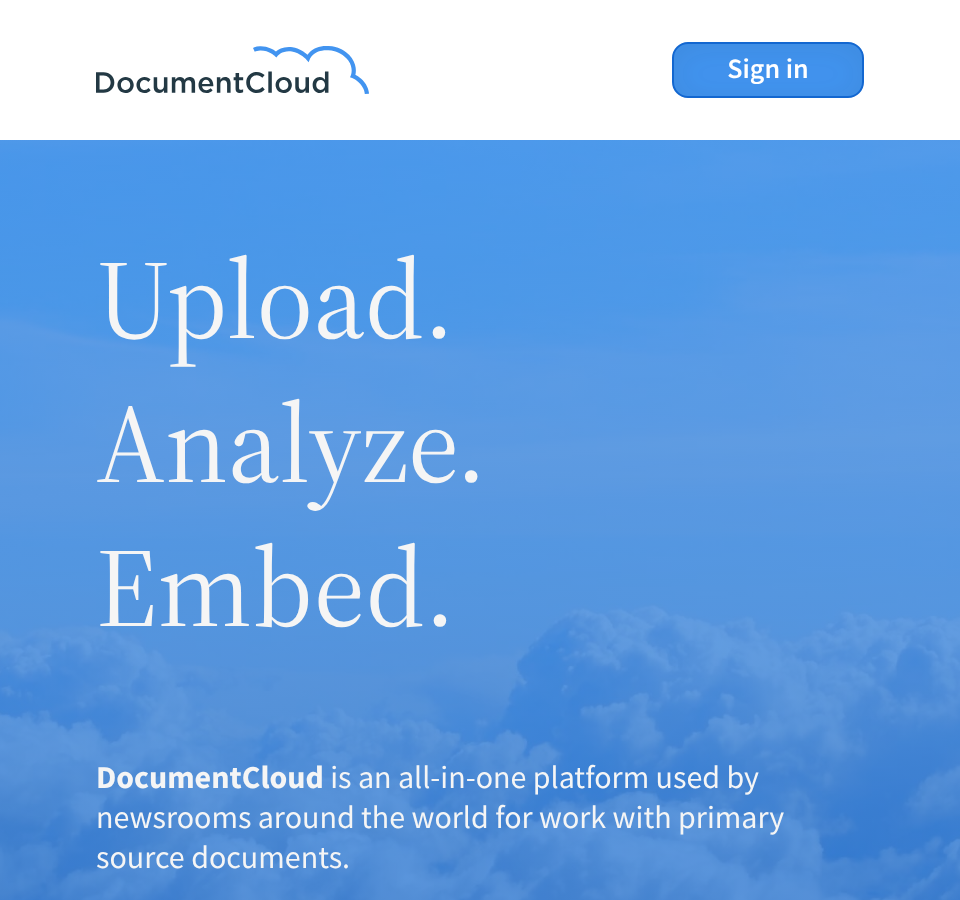
\includegraphics[width=\textwidth]{img/documentcloud.png}\\
            {\scriptsize DocumentCloud: shared infrastructure for analyzing document dumps.}
        \end{column}
    \end{columns}
\end{frame}

% Answer key (from data/ch-09/revenue-report-2024-12.pdf, checked 2026-10-12):
% the five 2024 sources sum to $171,006,200, but the printed subtotal is
% $171,006,199 -- the city's figures are rounded, so a check needs a tolerance.
% The subtotal's label wraps onto two lines. Page 15 (Exhibit 3) is a picture
% of a table under a note: nothing on it can be selected; Google Docs' OCR
% reads it. The 2023 column sums to $172,401,668, exactly the subtotal.
\begin{frame}{In class: the city's revenue report, by hand (20 minutes)}
    \begin{columns}[T]
        \begin{column}{0.6\textwidth}
            Work in pairs. Use no Python today.
            \begin{enumerate}\small
                \item Download Boulder's December 2024 revenue report from the textbook: \texttt{data/ch-09/revenue-report-2024-12.pdf}. (5 min)
                \item Get the \textbf{Sales and Use Tax Summary} on page 2 into a spreadsheet. Use copy and paste. Then use one other tool from the last three slides. (8 min)
                \item Clean it. Make one row per source, with the columns \texttt{source}, \texttt{2023}, and \texttt{2024}. Remove the \texttt{\$} signs and the commas. (4 min)
                \item Check it. Add the five sources for 2024. Compare the sum with the row ``Total Sales \& Use Tax based on current economic activity.'' (3 min)
            \end{enumerate}
            \smallskip
            {\small Fast? Try the same steps on page 15, Exhibit 3.}
        \end{column}
        \begin{column}{0.35\textwidth}
            \begin{block}{Report back}
                \small
                \begin{itemize}
                    \item Which route kept the rows and columns?
                    \item What did you fix by hand?
                    \item Did your sum match? If not, why not?
                \end{itemize}
            \end{block}
            \begin{block}{The file}
                \scriptsize \url{https://github.com/cuinfoscience/Web-Data-Science-Book/tree/main/data/ch-09}
            \end{block}
        \end{column}
    \end{columns}
\end{frame}

\begin{frame}{In the notebook}
    This week's companion notebook builds one skill at a time:
    \begin{itemize}
        \item \textbf{Setup} --- install pypdf, pdfplumber, pytesseract, and Tesseract, once
        \item \textbf{pypdf} --- a page's text in the order it was drawn, and the repairs it needs
        \item \textbf{pdfplumber} --- words and lines by where they sit on the page, and tables rebuilt from rules
        \item \textbf{OCR} --- text from a scan, or from a picture of a table
        \item \textbf{Checks} --- counts, sums, two tools, two documents, and a sample coded by hand
        \item \textbf{Case study 1} --- council minutes with pypdf: attendance and who spoke at Open Comment
        \item \textbf{Case study 2} --- revenue reports with pdfplumber: sales and use tax by year, 2017--2024
        \item \textbf{Document understanding} --- optional: AI parsers such as Docling, and Pandoc, judged with the same checks
    \end{itemize}
\end{frame}

% =========================================================================
\section{Wednesday · Notebook Lab}
% =========================================================================

\begin{frame}{Daily note questions}
    \begin{itemize}
        \item \textbf{Are these tools better than AI at extracting information from PDFs?} --- Definitely more painful, AI document understanding frameworks are what I would recommend
        \item \textbf{Why are PDFs standard?} --- Open standard, adoption, path dependence
        \item \textbf{How to read figures and charts?} --- OCR and extract text or use AI DU frameworks
        \item \textbf{Copying and pasting table into Excel} --- Use the Text-to-Columns button under Data tab
    \end{itemize}
\end{frame}

% The code on these frames is the chapter's (ch-09-pdfs.qmd, textbook PRs #258 and #261),
% shortened where a frame needs it; every output shown was printed by running it on the
% book's saved copies (data/ch-09/), on 2026-10-12 and 2026-10-14.
\begin{frame}[fragile]{Before the first cell: install once}
    \begin{columns}[T]
        \begin{column}{0.56\textwidth}
\begin{lstlisting}
%conda install -y -c conda-forge pypdf pdfplumber pytesseract tesseract
\end{lstlisting}
\begin{lstlisting}
import pypdf, pdfplumber, pytesseract
print(pypdf.__version__, pdfplumber.__version__)
print(pytesseract.get_tesseract_version())
# 6.20.1 0.11.10
# 5.5.3
\end{lstlisting}
        \end{column}
        \begin{column}{0.4\textwidth}
            \small A \texttt{webdata} made from today's setup page has all four. An older one, or Anaconda's \texttt{base}, needs the first cell; then restart the kernel.

            \medskip

            \texttt{pytesseract} is the Python library; \texttt{tesseract} is the OCR program it runs, and \texttt{pip} can't install it.
        \end{column}
    \end{columns}
\end{frame}

\begin{frame}[fragile]{pypdf: text in the order it was drawn}
\begin{lstlisting}
from pypdf import PdfReader

minutes_2024 = PdfReader(get_saved_copy("council-minutes-2024-12-05.pdf"))
text = minutes_2024.pages[0].extract_text()
# P age 1
# CI
# TY COUNCIL MEETING
# ...
# M
# ayor Brockett called the meeting to order at 6:00 p.m.
\end{lstlisting}
    Every word is there, and some are broken. Word drew the ``M'' of ``Mayor'', jumped to another line, and came back: pypdf starts a new line at each jump. \texttt{clean\_page\_text()} in the notebook removes ``P age 1'' and rejoins a first letter to the rest of its word.
\end{frame}

\begin{frame}[fragile]{The one line that flattens the page}
    \begin{columns}[T]
        \begin{column}{0.6\textwidth}
        Tempting one-liner:
\begin{lstlisting}
# DON'T: \s matches newlines too,
# so this flattens the whole page
re.sub(r'\s+', ' ', raw_text)
\end{lstlisting}
        Correct --- collapse spaces \& tabs, \textbf{keep} the line breaks:
\begin{lstlisting}
text = re.sub(r'[ \t]+', ' ', raw_text)
kept = []
for line in text.split('\n'):
    if line.strip():         # skip empty lines
        kept.append(line.strip())
clean = '\n'.join(kept)
\end{lstlisting}
        \end{column}
        \begin{column}{0.35\textwidth}
            The most important choice is what \textit{not} to collapse.

            \bigskip

            Line structure is real information: a roll call's names, and each Open Comment entry, sit on lines of their own.

            \bigskip

            Erase the newlines and no pattern can find where an entry starts.
        \end{column}
    \end{columns}
\end{frame}

\begin{frame}[fragile]{pdfplumber: words where they sit}
    \begin{columns}[T]
        \begin{column}{0.46\textwidth}
\begin{lstlisting}
import pdfplumber

with pdfplumber.open(report_2024) as report:
    page = report.pages[1]
    tables = page.find_tables()
    rows = tables[0].extract()
print(rows[-1][:2])
# ['Use Tax Audit Revenue', None]
\end{lstlisting}
            \small pdfplumber groups characters by \textbf{position}, so ``Mayor'' comes out whole. Its table finder rebuilds a grid from the page's rules. On the December 2024 summary page it stops one row short: the \textbf{total} has no vertical rules beside it, and nothing raises an error.
        \end{column}
        \begin{column}{0.5\textwidth}
            \centering
            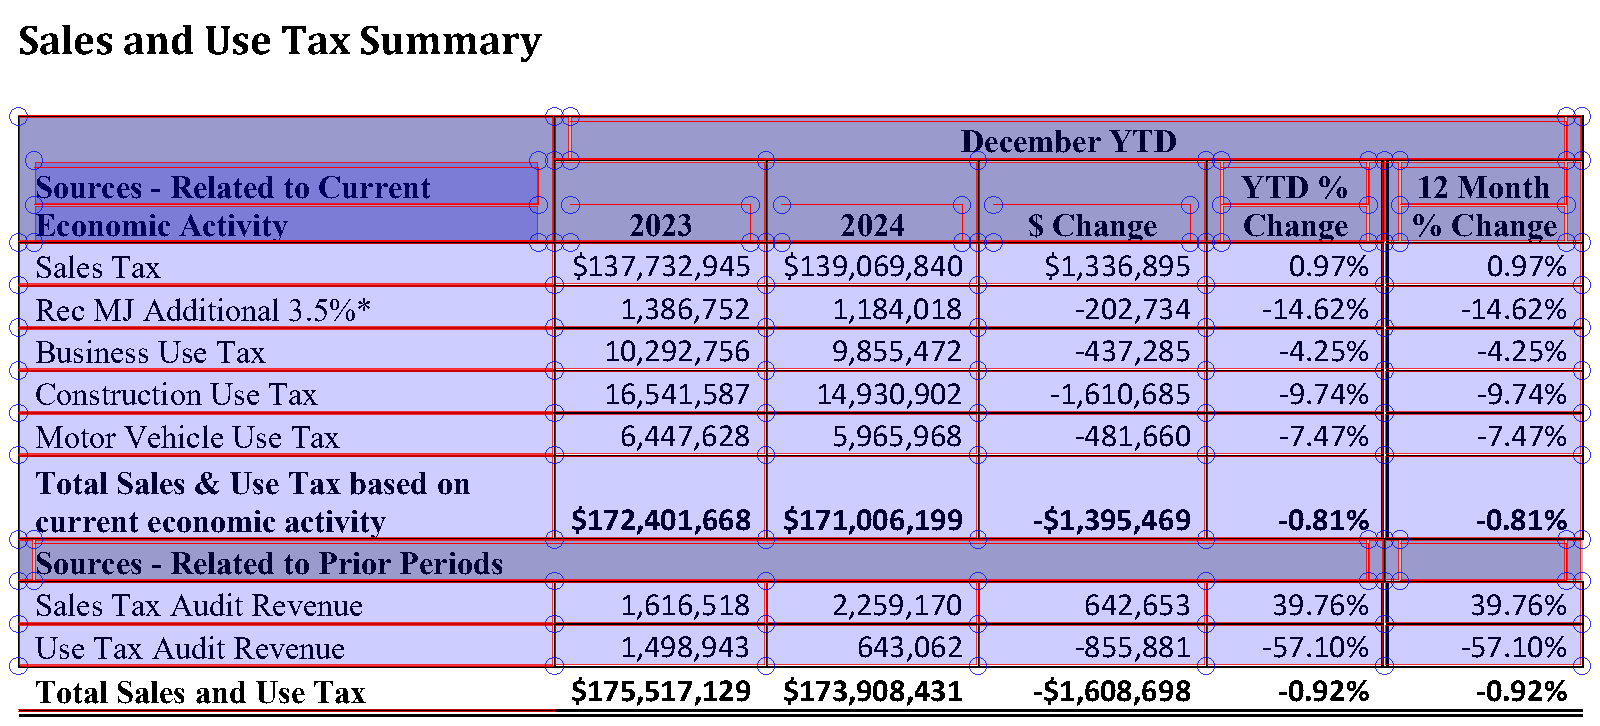
\includegraphics[width=\textwidth]{img/missing_totals_row.png}\\
            {\scriptsize pdfplumber's table finder on the summary page: shaded where it found cells. The total, at the bottom, is left out.}
        \end{column}
    \end{columns}
\end{frame}

\begin{frame}{pdfplumber's table settings}
    \texttt{find\_tables()} and \texttt{extract\_table()} take one dictionary of settings:
    \begin{itemize}\small
        \item \textbf{Strategies}: \texttt{"lines"} (rules and rectangle sides, the default), \texttt{"lines\_strict"}, \texttt{"text"} (words that line up), \texttt{"explicit"} (positions you give).
        \item \textbf{\texttt{explicit\_vertical\_lines}}: the column edges yourself, as the chapter does to get the totals row back.
        \item \textbf{Tolerances}, 3 points each: \texttt{snap} (merge near-parallel rules), \texttt{join} (join broken rules), \texttt{intersection} (where rules cross), \texttt{edge\_min\_length} (drop short marks).
        \item \textbf{Text strategy}: \texttt{min\_words\_vertical} (3), \texttt{text\_x\_tolerance}.
        \item \textbf{See it}: \texttt{page.to\_image().debug\_tablefinder(settings)}.
    \end{itemize}
    \medskip
    \centering\small All of them, with defaults: \url{https://github.com/jsvine/pdfplumber\#table-extraction-settings}
\end{frame}

\begin{frame}[fragile]{No text layer: OCR}
    \begin{columns}[T]
        \begin{column}{0.5\textwidth}
\begin{lstlisting}
import pytesseract

exhibit_3 = (PdfReader(report_2024)
    .pages[14].images[0].image.convert("L"))
ocr_text = pytesseract.image_to_string(
    exhibit_3, config="--psm 6")
# 2021 8,059,343 7,608.759 10,351,245 ...
\end{lstlisting}
            \small Exhibit 3 of the December 2024 report is a \textbf{picture} of a table. Tesseract reads it, and puts periods for commas in a few figures. The rows' sums catch every misread digit; Tesseract's confidence scores don't.
        \end{column}
        \begin{column}{0.46\textwidth}
            \centering
            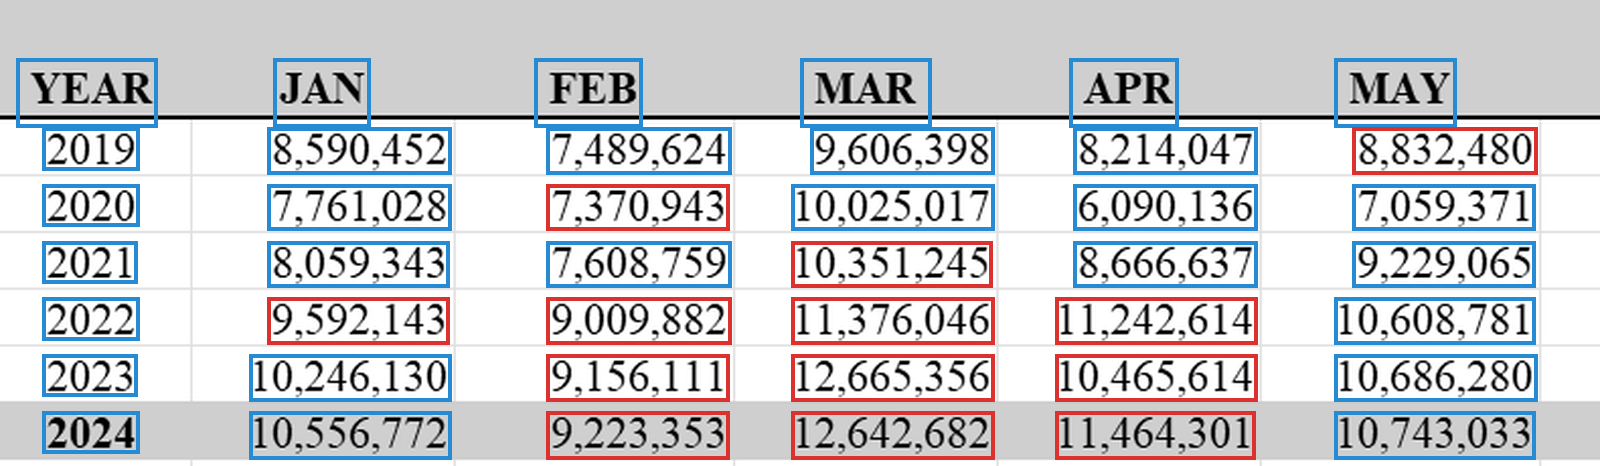
\includegraphics[width=\textwidth]{img/ocr_confidence.png}\\
            {\scriptsize Each word Tesseract read: blue if its confidence is 80 or more, red if less. Most red words are right.}
        \end{column}
    \end{columns}
\end{frame}

\begin{frame}{Check every extraction}
    Extraction fails without errors. Each of these caught a real problem in Chapter 9:
    \begin{enumerate}\small
        \item \textbf{Look at the page beside the output.}
        \item \textbf{Count.} The summary table has nine rows of figures; the council has nine seats.
        \item \textbf{Sums.} The five sources add up to \$171,006,200; the printed subtotal is \$171,006,199.
        \item \textbf{Two tools agree.} pypdf's and pdfplumber's text give the same speaker counts.
        \item \textbf{Two documents agree.} A year printed in two reports should match.
        \item \textbf{A sample coded by hand.} Read some pages yourself, and measure the extraction against them.
    \end{enumerate}
\end{frame}

\begin{frame}[fragile]{Case study 1: the obvious regex}
    \begin{columns}[T]
        \begin{column}{0.6\textwidth}
\begin{lstlisting}
present = re.search(r'Present:\s*(.*?)\s*(?:Absent:|$)',
                    page_1, re.IGNORECASE | re.MULTILINE)
\end{lstlisting}
            Eleven December meetings, 2018--2024, read with pypdf. This pattern finds \textbf{nobody} in the five meetings before 2022, and \textbf{5 of 9} members after.

            \medskip

            The minutes recorded the roll call two ways:
            \begin{itemize}\small
                \item through 2020, a sentence: ``Council Members Brockett, \ldots{} and Young were present.'' The mayor isn't in it.
                \item from 2021, a label and a list that wraps onto a second line, with a separate label for members online.
            \end{itemize}
        \end{column}
        \begin{column}{0.35\textwidth}
            \centering
            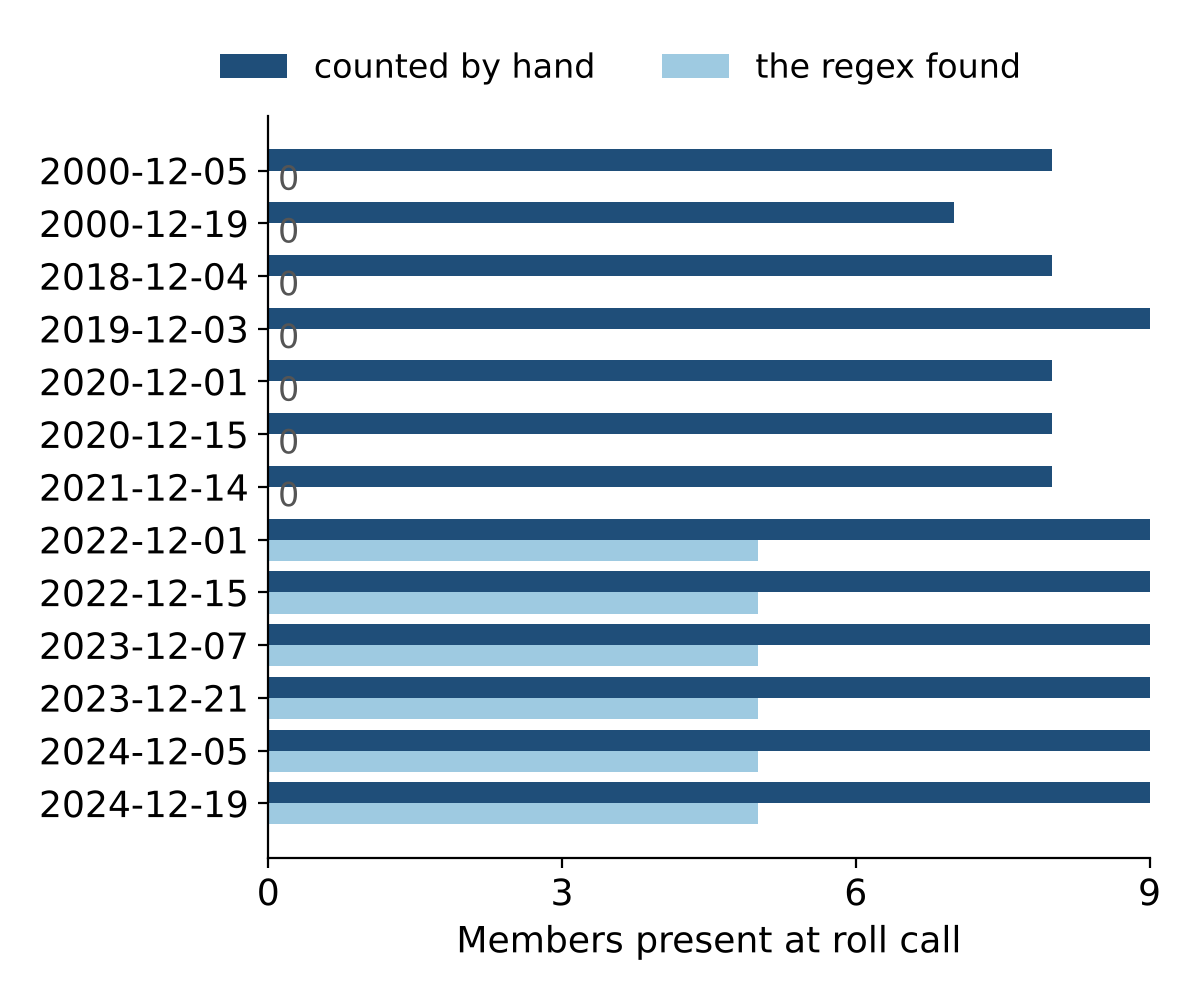
\includegraphics[width=\textwidth]{img/attendance_chart.png}\\
            {\scriptsize Members present at roll call, with the two December 2000 scans: counted by hand (dark), and found by this regex (light).}
        \end{column}
    \end{columns}
\end{frame}

\begin{frame}[fragile]{Case study 1: one function, both formats}
\begin{lstlisting}
def roll_call(page_1):
    present = set()
    mayor = re.search(r"Mayor (\w+) called the meeting to order", page_1)
    if mayor:
        present.add(mayor.group(1))
    # 2018-2020: "Council Members Brockett, ... and Young were present"
    sentence = re.search(r"Council Members ([A-Z][^:]*?)\s+were\s+present", page_1)
    if sentence:
        present |= split_names(sentence.group(1))
    # 2021-2024: "Council Members present:", "Virtually present:", "Present virtually:"
    ...   # each list, plus the next line while the list ends with a comma
    return present
\end{lstlisting}
    \small It matches a hand count of all eleven meetings: 8 or 9 members at each roll call. A member who arrived late counts as absent, and one member is ``Swetlik'' in 2019 and ``Swetlick'' in 2020.
\end{frame}

\begin{frame}[fragile]{Case study 1: who spoke at Open Comment}
    \begin{columns}[T]
        \begin{column}{0.48\textwidth}
\begin{lstlisting}
ENTRY_START = re.compile(
    r"^[\dlJt](?: ?[\dlJt])? ?\.? +[A-Z]"
    r"|^[A-Z]\S* .*?\b(?:s ?poke|"
    r"signed up|withdrew)\b")
DID_NOT_SPEAK = re.compile(
    r"did not|withdr|not present"
    r"|duplicate|moved to", re.I)
\end{lstlisting}
            \small An entry starts at a list number, as the 2018--19 scans' OCR misreads it (``l0'', ``J''), or at a name followed by ``spoke''. Four tries to get there. It counts; it never prints a name.
        \end{column}
        \begin{column}{0.48\textwidth}
            \centering
            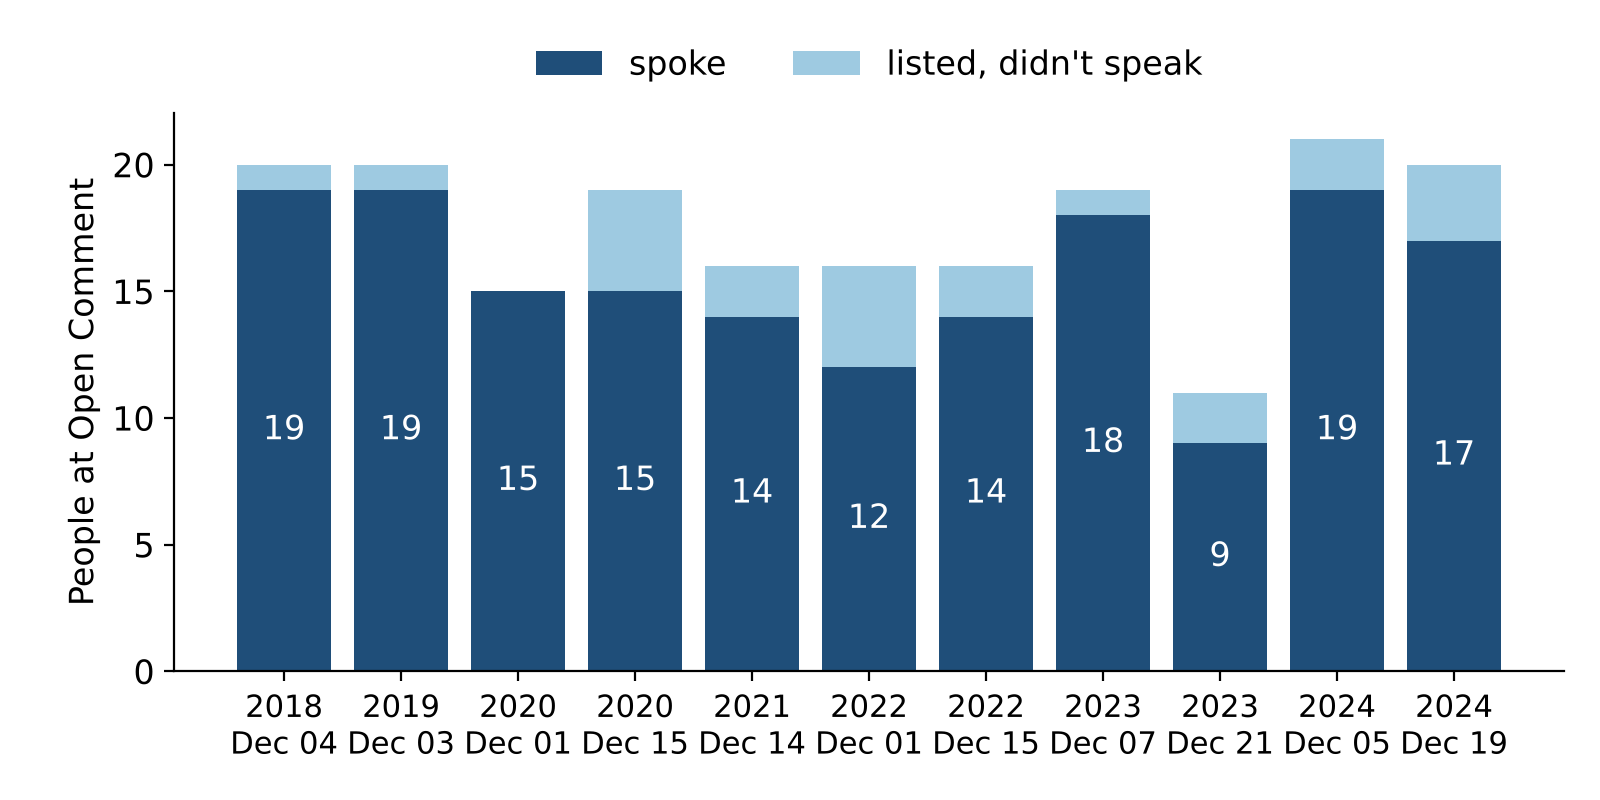
\includegraphics[width=\textwidth]{img/open_comment.png}\\
            {\scriptsize Residents who spoke at Open Comment, December meetings 2018--2024. Lighter: listed, but didn't speak.}
        \end{column}
    \end{columns}
\end{frame}

\begin{frame}[fragile]{Case study 2: read the totals row by position}
\begin{lstlisting}
def row_words(page, label):
    found = page.search(label)[0]        # where the label sits, in points
    # a strip of the page, as tall as the label's line
    line = page.crop((0, found["top"] - 1, page.width, found["bottom"] + 1))
    words = []
    for word in line.extract_words():
        if word["x0"] > found["x1"]:     # right of the label
            words.append(word["text"])
    return words

row_words(page, "Total Sales and Use Tax")   # the 2018 report
# ['$134,538,892', '$140,648,710', '$6,109,818', '4.54%']
\end{lstlisting}
    \small Seven year-end revenue reports. Find the summary page by its text: 2020's report opens with a letter restating earlier figures, so its summary is on page 3. Then skip the table finder, and read the one row you need by where it sits. Each report's own change column checks the two totals.
\end{frame}

\begin{frame}{Case study 2: one series from seven reports}
    \begin{columns}[T]
        \begin{column}{0.46\textwidth}
            Six years are printed twice: in their own report, and as ``the year before'' in the next. Five agree to the dollar.

            \medskip

            \textbf{2018 doesn't.} The 2019 report gives it as \$38,959 less than the 2018 report did, and doesn't say why. Use each year's latest printing, and say so.

            \medskip

            Sales and use tax fell \textbf{4.76\%} in 2020, then rose \textbf{12.65\%} and \textbf{11.04\%}. In dollars of each year: not adjusted for inflation.
        \end{column}
        \begin{column}{0.5\textwidth}
            \centering
            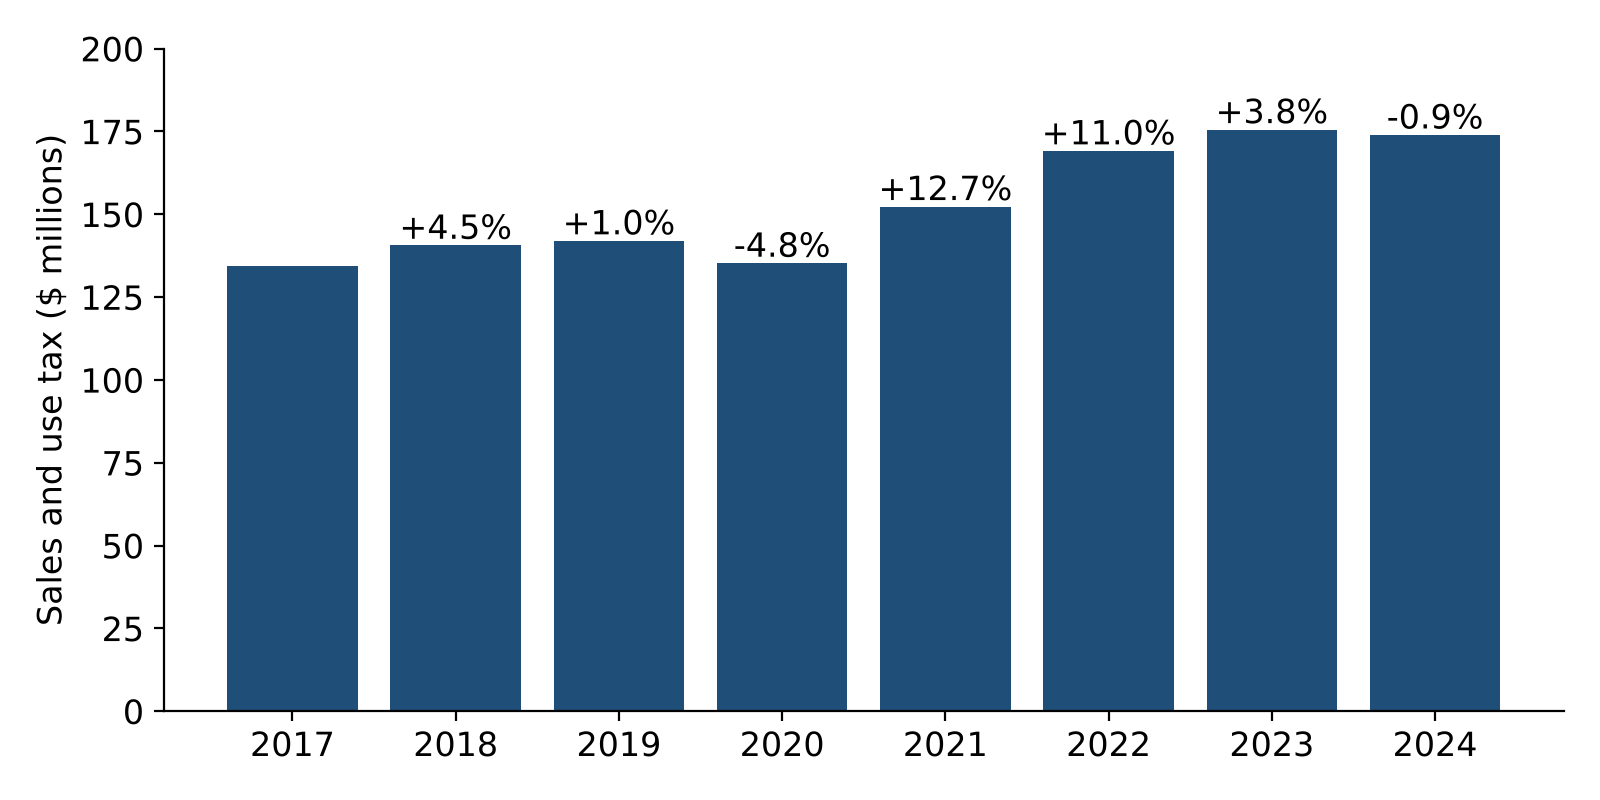
\includegraphics[width=\textwidth]{img/sales_use_tax.png}\\
            {\scriptsize Total sales and use tax by year, read with pdfplumber, with the change from the year before.}
        \end{column}
    \end{columns}
\end{frame}

\begin{frame}{Document understanding: AI parsers, optional}
    \begin{columns}[T]
        \begin{column}{0.52\textwidth}
            \begin{itemize}\small
                \item \textbf{Text-layer converters}: MarkItDown. Fast; a scan gives it nothing.
                \item \textbf{Pipelines}: layout + table + OCR models. Docling runs on a laptop.
                \item \textbf{Vision-language models}: olmOCR, DeepSeek-OCR, Datalab's Chandra. Most need a GPU, or a hosted service that receives your file.
                \item \textbf{Pandoc} converts the Markdown they write to HTML or Word. It can't read a PDF.
            \end{itemize}
            \medskip
            \footnotesize None of these is in \texttt{webdata} or needed for the lab: Chapter 9, ``Document Understanding.''
        \end{column}
        \begin{column}{0.44\textwidth}
            \small \textbf{Docling on Exhibit 3}, the picture of a table:
            \begin{itemize}\small
                \item 21 of 30 rows whole, and each adds up
                \item 9 incomplete or merged; 2 under the wrong label
                \item no error raised
            \end{itemize}
            \medskip
            Same checks as ever: count, sums, labels, two tools.
        \end{column}
    \end{columns}
\end{frame}

\begin{frame}{Lab: work these, then show-and-tell}
    \begin{columns}[T]
        \begin{column}{0.6\textwidth}
            Work in pairs. Run both case studies in the notebook, then extend one:
            \begin{enumerate}\small
                \item Run \texttt{roll\_call()} on the two December 2000 minutes. They are scans. What does the pattern miss? Fix it, and check against the page.
                \item Count the votes in each meeting with the tally pattern (\texttt{Carried 9:0}). What share were unanimous?
                \item Code one meeting's Open Comment list by hand. Compare your count with the function's.
                \item Read the \textbf{Sales Tax} row from all seven reports with \texttt{row\_words()}. Plot it beside the total.
                \item Read the 2023 summary table with \texttt{find\_tables()}. Which rows does it find? Compare with \texttt{row\_words()}.
                \item[6.] \textbf{5617}: write a memo about the two datasets you built. Use the categories of \textcite{gebru2021datasheets}
            \end{enumerate}
        \end{column}
        \begin{column}{0.35\textwidth}
            \begin{block}{Show-and-Tell}
                \footnotesize Bring one of these to class:
                \begin{itemize}\footnotesize
                    \item a bug that you could not solve
                    \item data that you collected and find interesting
                    \item a question for a research design
                \end{itemize}
            \end{block}
        \end{column}
    \end{columns}
\end{frame}

% =========================================================================
\section{Friday · Textbook Revisions}
% =========================================================================

% The screenshot's code is 12 CSS pixels; a 62% column brings it to 16 on a
% slide shown 1,920 pixels wide (slides/common/AUTHORING.md), and 60% would not.
\begin{frame}{Improving Chapter 9 together}
    \begin{columns}[T]
        \begin{column}{0.62\textwidth}
            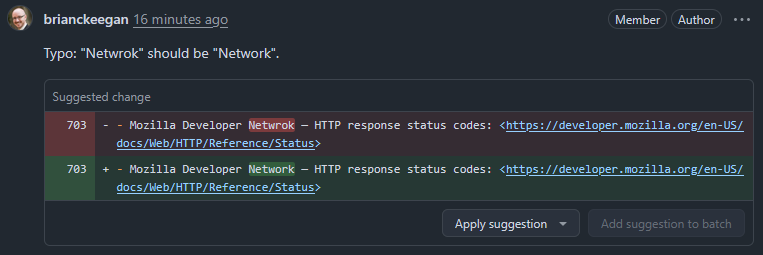
\includegraphics[width=\textwidth]{img/pr_suggestion.png}

            \medskip

            Today we make the book better. Each of you opens a \textbf{pull request} against \texttt{ch-09-pdfs.qmd} and reviews a classmate's.
        \end{column}
        \begin{column}{0.33\textwidth}
            The workflow (from Week 1):
            \begin{enumerate}\small
                \item Branch / fork the book repo
                \item Edit the chapter; commit with a clear message
                \item Open a PR describing \textit{what} and \textit{why}
                \item Review two peers' PRs: kind, specific, actionable
            \end{enumerate}
        \end{column}
    \end{columns}
\end{frame}

\begin{frame}{A revision menu for Chapter 9}
    High-value targets --- pick one and scope it to a single PR:
    \begin{itemize}
        \item \textbf{Run it against real Boulder minutes.} The \texttt{\# Returns:} outputs and five regex patterns are \textit{illustrative}. Download actual signed minutes, report what the patterns catch and miss, and label sample output as representative.
        \item \textbf{Add the chapter's first figures.} It is all code and prose today: a ``drawing-instructions vs.\ logical text'' diagram, a pipeline flowchart, or an annotated minutes screenshot would anchor Monday's core idea.
        \item \textbf{Harden \texttt{extract\_attendance}.} The chapter itself flags ``Absent: None,'' title variants (``Council Member Smith''), and semicolon / line-break separators. Contribute handling \textbf{plus tests} for the formats you actually hit.
        \item \textbf{Make an exercise self-checking.} Add expected output, a rubric, or a starter cell to the open-ended ``find and extract'' and ``topic tracking'' exercises.
        \item \textbf{Deepen ``When PyPDF Is Not Enough.''} Turn the two-line \texttt{pdfplumber} / OCR sketches into a runnable table-extraction or Tesseract example tied to ``Further Reading.''
    \end{itemize}
\end{frame}

\begin{frame}{A good revision, and a good review}
    \begin{columns}[T]
        \begin{column}{0.6\textwidth}
            \begin{block}{A strong PR}
                \begin{itemize}\small
                    \item One focused change, clearly titled
                    \item Explains the problem it fixes
                    \item Builds (\texttt{quarto render}) without errors
                    \item Matches the book's voice and notation
                    \item Discloses any AI assistance
                \end{itemize}
            \end{block}
        \end{column}
        \begin{column}{0.35\textwidth}
            \begin{block}{A strong review}
                \begin{itemize}\small
                    \item Runs / reads the change, not just skims
                    \item Names specifics (line, claim, code)
                    \item Separates ``must fix'' from ``nice to have''
                    \item Is generous --- assume good faith
                    \item Ends with a clear verdict
                \end{itemize}
            \end{block}
        \end{column}
    \end{columns}
    \medskip
    \centering\small Next week: a new module on \textbf{APIs} --- when data arrives as JSON and no parsing is required (starting with Wikipedia).
\end{frame}

% =========================================================================
\begin{frame}{Key takeaways}
    \begin{enumerate}
        \item PDFs optimize \textbf{visual fidelity over structure} --- extraction is reconstruction, not reading.
        \item \texttt{pypdf} gives text in the order it was drawn; expect breaks inside words and plan to clean them.
        \item Collapse spaces/tabs but \textbf{keep newlines} --- line structure is information; regex imposes the rest.
        \item \texttt{pdfplumber} keeps each word's position: find a label, then read its row. OCR is for pages with no text layer.
        \item \textbf{Check every extraction} against a count by hand or a total the document prints --- across all its formats.
    \end{enumerate}
    \bigskip
\end{frame}

\end{document}
